
\subsection{Uncertain Injects}
\begin{frame}{Uncertain Injects}
\alert{Uncertainty in Injects to Power System}
\bi
\item Subset of nodes have uncertain injections
\bi
\item Solar, wind
\item Demand (relatively certain, however EVs could represent change)
\ei
\pause
\item Subset of assets respond to uncertainty (slack distribution)
\bi
\item Rotational inertia, peaker plants and regulation
\item Energy storage, enhanced power controls
\ei
\ei
\end{frame}


\begin{frame}{Uncertainty is Multivariate Normal}
\alert{Assumption}

Uncertainty in net injections are Multivariate Normal
\bi
\item \textit{Uncertainty in errors from forecast}
\item Known or can be empirically estimated
\item Potentially correlated
\ei
\begin{center}
% 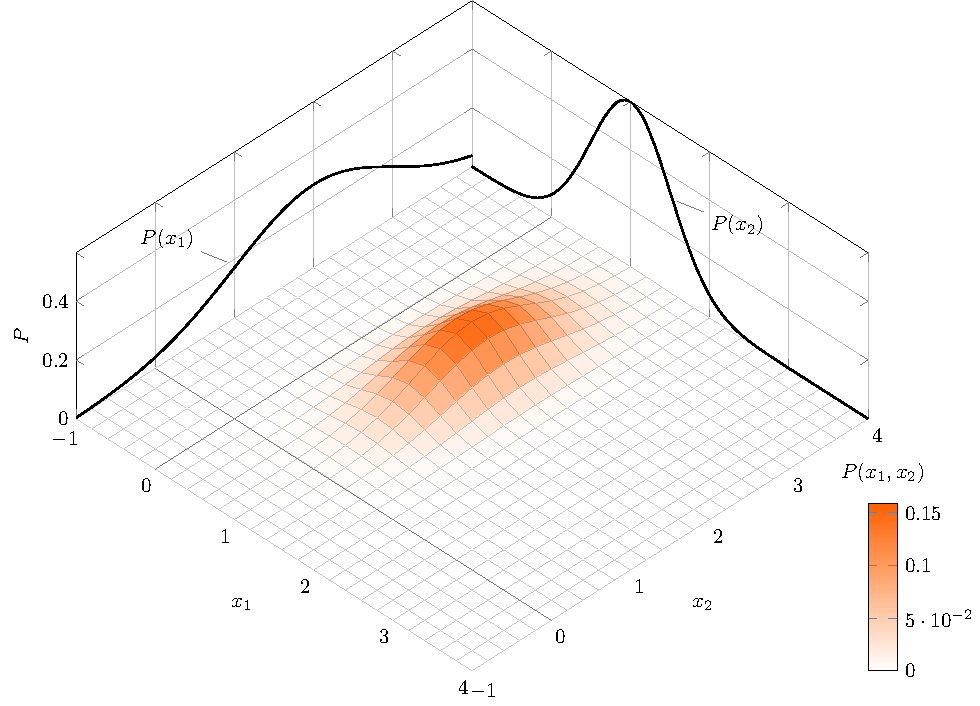
\includegraphics[scale=.325]{multivariate} 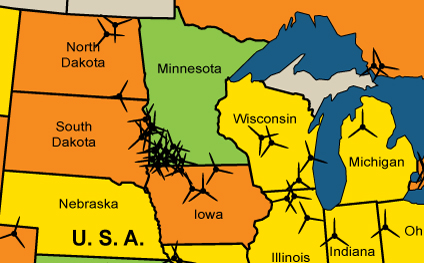
\includegraphics[scale=.35]{windmap}
\begin{figure}
   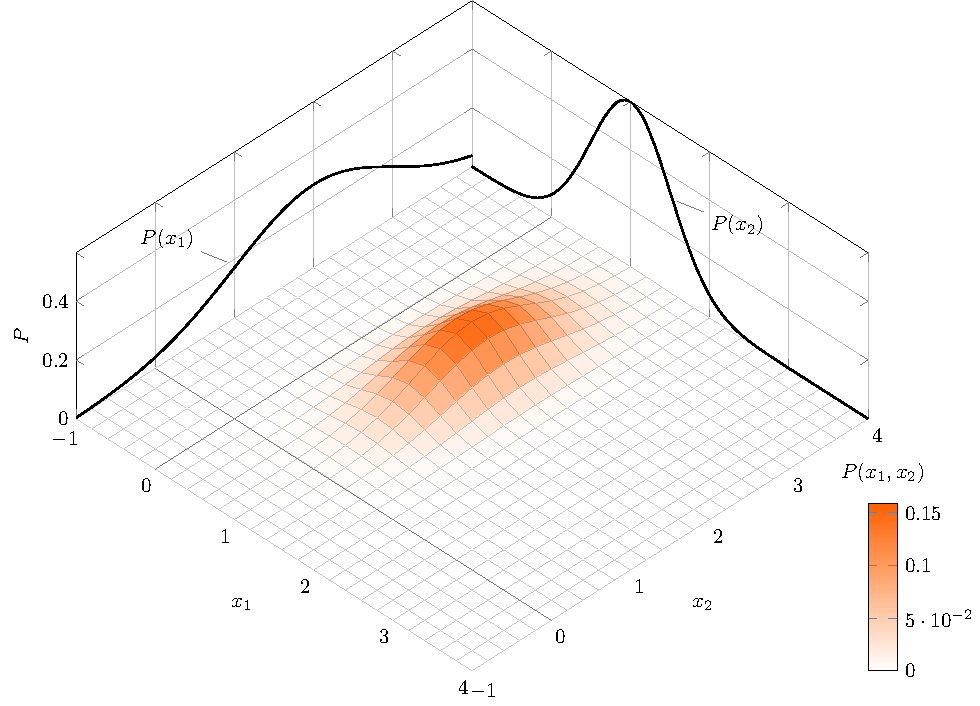
\includegraphics[width=0.475\textwidth]{multivariate}
   \hfill
   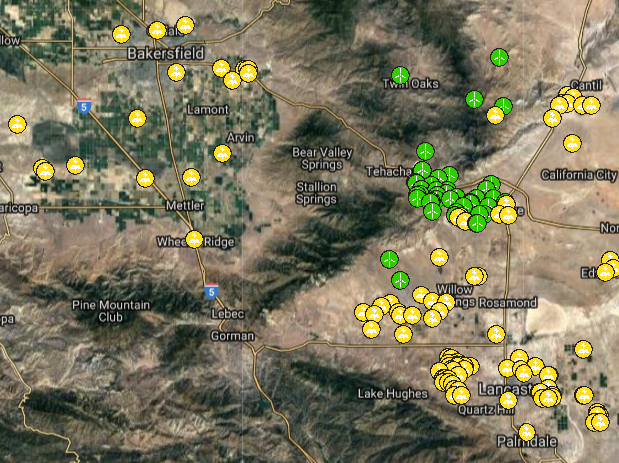
\includegraphics[width=0.475\textwidth]{renewables-correlated}
\end{figure}
\end{center}
%Error from short term forecast for windfarms is normally distributed

\end{frame}


\begin{frame}{Gaussian Injects}
\alert{Net Injection Uncertainties}
\bi
\item Subset of nodes have uncertain injections (i.e. wind)
\item Subset of generators respond to uncertainty (slack distribution)
\ei
\pause
\begin{equation*}
 \rx = C_g\left(\alert{x_g}+\rD\alert{\beta}\right) - (d + C_M \ri) 
\end{equation*}

\pause
\begin{tabular}{ c l}
$\rx$ & Net injects \\
$x_g$ & Generator dispatch \\
$\beta$ & Slack distribution \\
$d$ & Expected demand \\
$\ri$ & Nodal demand variation ($\mathbb{E} \left[ \ri \right] = 0$, $\Sigma$ known)\\
$\rD$ & Aggregate demand variation ($\rD = 1^T \rdm$)
\end{tabular}
\end{frame}


\begin{frame}{Gaussian Branch Flows}
Assuming Gaussian injects and linear shift factors
\bi
\item Branch flows are Gaussian as well
\ei
\pause
\begin{equation*}
 \ry = \alert{y_0}+ A C_G\alert{ \beta }\rD  - A C_M \rdm 
\end{equation*}
\pause
\begin{tabular}{c l}
$\ry$ & Branch flows \\
$y_0$ & Branch flows for forecasted system \\
$A C_g \beta \rD$ &  Flow variation due to slack generation movement \\
$A C_m \rdm $ & Flow variation due to nodal inject changes
\end{tabular}

%Random component of branch flow
%\begin{equation*}
%\rf = A C_G \beta \rD - AC_M \ri
%\end{equation*}
\end{frame}




\subsection{Issues with Deterministic Analysis}
\begin{frame}{Issues with Deterministic Analysis}
Normal distributed injects 
\pause 
$\rightarrow $
\textbf{Normal branch flows}\footnotemark
\vspace{20px}
\footnotetext[1]{In a stable system}
\pause
\alert{Problem!}
\bi
\item Branch constraints violated half the time when at its limit
\ei
\end{frame}

\begin{frame}{Normal Branch Flow}
\begin{center}
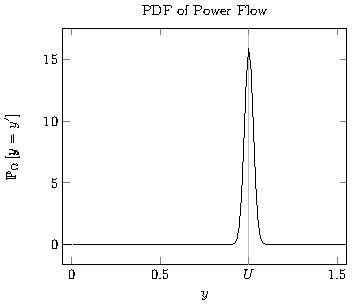
\includegraphics[scale=1.1]{fig-ccflow}
\end{center}
PDF for Branch flow with mean (forecast) at nominal capacity
\end{frame}


\begin{frame}{Normal Branch Flow}
\begin{center}
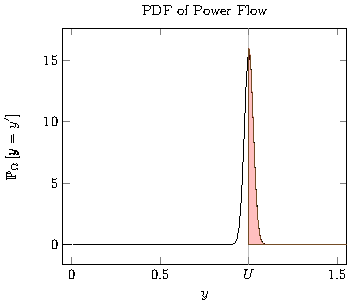
\includegraphics[scale=1.1]{fig-ccflowred}
\end{center}

\alert{Need to probabilistically enforce constraints}

\end{frame}


\subsection{Chance Constraints}

\begin{frame}{Chance Constraint Model}
Replace the standard constraints with probalistic ones \footnotemark \footnotemark
\[ P \left[ -U_e \leq \ry_e \leq U_e \right] \geq 1- \epsilon_l \hspace{20pt} \forall e\] 

\pause
\alert{Deterministic equivalent}


%Generators 
%\[ x_j + \beta_j \sigma_\Delta \eta_g \in \left[ G^{min}_j, G^{max}_j \right] \hspace{10pt} \forall j     \]
%\pause
Branch flows
\[ y_e + s_e \eta_l \leq  U_e  \hspace{30pt} \forall e    \]
with
%\[ \eta_g = \Phi^{-1}(1 - \epsilon_g) \]
\[ \eta_l = \Phi^{-1}(1 - \epsilon_l) \]


\footnotetext[1]{{Bienstock}, D. and {Chertkov}, M. and {Harnett}, S.}
\footnotetext[2]{Vrakopoulou, M. and Chatzivasileiadis, S. and Andersson, G.}

%and 
%\begin{align*}
% s^2_e &= \pi_e^2 \sD - 2 \pi_e \se  +\see \\
%\pe &= \textstyle \sum_j A_{ej} \beta_j 
%\end{align*}

%\begin{alignat*}{3}
%                 && \pe - \textstyle \sum_j A_{ej} \beta_j   &=0 &&\forall e \\ 
%                 && s^2_e - \pi_e^2 \sD + 2 \pi_e \se      &\geq\see &&\forall e  \\
%                 && \textstyle \sum_j \beta_j &=1 &&
%\end{alignat*}




\end{frame}


\begin{frame}{Chance Constraints}

\begin{center}
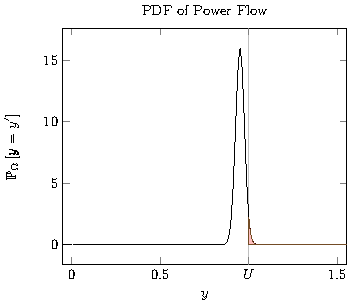
\includegraphics[scale=1.1]{fig-ccflowred-95}
\end{center}


\end{frame}
